\documentclass[conference, 11pt, onecolumn]{IEEEtran}

\usepackage{blindtext, graphicx}
\usepackage[justification=centering]{caption}

\hyphenation{op-tical net-works semi-conduc-tor}

\begin{document}

\title{Weakly Supervised Training of Noisemes}

\author{
\IEEEauthorblockN{Tianyu Xu}
\IEEEauthorblockA{Carnegie Mellon University\\
School of Computer Science\\
Language Technologies Institute\\
Email: tianyux@andrew.cmu.edu}
\and
\IEEEauthorblockN{Liping Xiong}
\IEEEauthorblockA{Carnegie Mellon University\\
School of Computer Science\\
Language Technologies Institute\\
Email: lipingx@andrew.cmu.edu}
}

%\IEEEspecialpapernotice{(Invited Paper)}

\maketitle

\begin{abstract}
In this paper, we present a novel approach to enlarge noiseme training dataset inspired by the idea of co-training. Given videos with automatically generated noiseme labels and image concepts, we introduce three different methods to discover stable correlations between sounds and images, and use corresponding image concepts as the evidence to support the automatically labeled noisemes based on insightful correlations. We propose several ways to fuse and refine the found correlations. Also, we construct new training datasets in two different ways, and conduct several experiments to show that the proposed approach is able to effectively select new training samples from automatically labeled data, and weakly supervised training can help improve the accuracy of noiseme detectors.
\end{abstract}

\begin{IEEEkeywords}
noiseme, co-training, multimedia analysis.
\end{IEEEkeywords}

\section{Introduction}
\label{section:introduction}
Noiseme, as described in \cite{burger2012noisemes}, is the smallest segmental unit of sound employed to form meaningful contrasts between noises. Noiseme labels describe distinct noise units based on audio concepts, independent of visual concepts as much as possible. They are useful for many multimedia analysis tasks such as multimedia event detection and detailed summaries of videos. We can create event signatures or event fingerprints using particular noiseme patterns or significant noiseme co-occurrences from different modalities.

In order to build accurate noiseme detectors, a large-scale manually labeled training set is needed. However, current noiseme classifiers were only trained on 5.6 hours of manually labeled audio data, which is not sufficient and leaves much room for performance improvements. We want to find a way to leverage the 6,000 hours videos we have now, although they do not have manually labeled noiseme information, and let them contribute to the training process as well. To achieve this goal, we can use the noiseme detectors trained by manually labeled data to label the 6,000 hours unlabeled data, and select reliable noiseme snippets as new samples to enrich the training set.

We hold the assumption that some noisemes can be "seen" in the corresponding video. For example, if we see a dog appears in a video, we are likely to hear barking at the same time. Similarly, if we see a vehicle drives through the street, we will probably hear the engine sound fade in and fade out. Holding the assumption that some noisemes are correlated with some image concepts, we can find informative noiseme-image correlation pairs and use the image concepts as the evidence to support automatically generated noiseme labels. Then we select verified noiseme features from automatically labeled data to enlarge the training set and re-train the models.

We propose the weakly supervised training approach as four phases. First, we describe three different correlation discovering methods which can find correlation pairs, i.e. find noiseme labels and image concepts that co-occur frequently. Second, we introduce a straightforward late fusion process to combine correlation discovering results. Third, we refine the resultant correlations from two different aspects: eliminate inaccurate automatically generated labels and take advantage of image concept hierarchy to merge similar image concepts. Fourth, we describe how to construct a new training set based on the correlations we get.

The rest of the paper is organized as follows. In Section \ref{section:data}, we give an overview of the datasets we have, including the manually labeled set and the much larger set with automatically generated labels, and the low-level acoustic features we use in noiseme classifier training. In Section \ref{section:methods}, we provide details of the proposed approach and show how to find informative correlations and build new training set based on them. In Section \ref{section:experiments} and Section \ref{section:results}, we discuss the experiments we conducted and analyze the results. At last, we give our conclusions and indicate who contributed which part of the project.

\section{Data and Features}
\label{section:data}
We have two different datasets. The first dataset is the one manually labeled with noiseme labels, and its duration is 5.6 hours. The human ear is fairly good in identifying sounds so we can take these manually labeled noisemes as ground truth. The second dataset is the one with automatically generated noiseme labels and image concepts. The total duration of this dataset is more than 6,000 hours. We have 1,000 different image concepts, which were labeled by a koala model. For each video, several keyframes were selected and labeled with these image concepts. Also, we have 40 different noiseme labels, which were labeled by a random forest model. Note that the number of noiseme labels is not consistent with the number we provided in Section \ref{section:introduction}, because some noisemes only appear in several clips so that we filtered them out. A fixed length (100ms) sliding window slides from the beginning to the end and labels are given by the noiseme detectors trained on the manually labeled dataset. The format of each video is shown in Figure \ref{fig:format}.

\begin{figure}[h!]
\centering
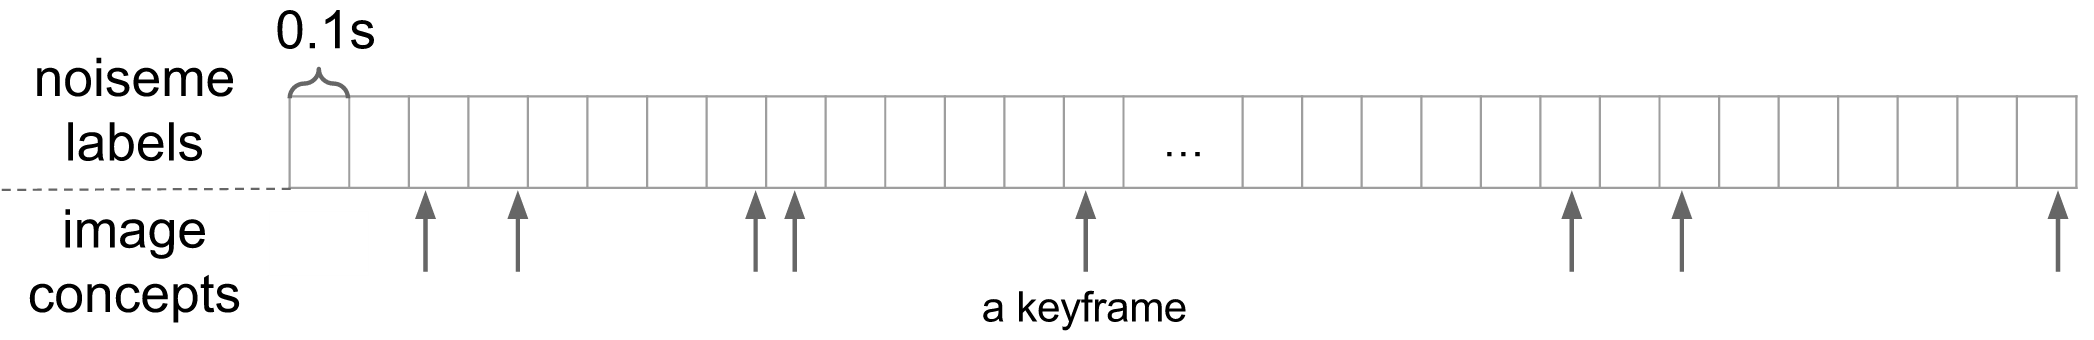
\includegraphics[scale=0.45]{figure/format.png}
\caption{The format of videos in the automatically labeled dataset.}
\label{fig:format}
\end{figure}

We use features described in \cite{wang2014exploring} as low-level features. First, standard acoustic features are extracted using the toolkit openSMILE \cite{eyben2013recent} (speech and music interpretation by large space extraction), and then we apply a set of statistical functions over these acoustic features within the fixed length sliding window to get the final representations. The dimension of the feature vector is $983$. The feature set is listed in Table \ref{table:features}.

\begin{table}[h]
\normalsize
\begin{center}
\caption{Feature set list, cited from \cite{wang2014exploring}.}
\label{table:features}
\begin{tabular}{| c | p{10cm} |}
\hline
MFCC (13 + 13 delta + 13 delta delta) & arithmetic mean, standard deviation, linear regression parameter, quartiles, range \\
\hline
MFC (26 + 26 delta) & The same set with log-energy + kurtosis \\
\hline
Log-energy & quadratic mean (non-zero value), standard derivation, max Pos, min Pos, linear regression parameter, quartiles, range \\
\hline
F0 & quadratic, standard deviation, maximum mean, minimum mean, linear regression, qiartiles, range \\
\hline
\end{tabular}
\end{center}
\end{table}

\section{Methods}
\label{section:methods}

\subsection{Correlation Discovering}
We proposed three different approaches to discover the insightful correlation pairs, i.e. find noiseme labels and image concepts that co-occur frequently. All the approaches are based on statistical models and we no prior knowledge is required toward the correlations.

\subsubsection{Score multiplication}
The first approach is the most straightforward approach. Automatically generated noiseme labels and automatically generated image concepts are both assigned with confident scores range from $[0, 1]$. For each noiseme - image concept pair, we can simply multiply their confident scores as the \emph{correlation score} towards the correlation pair, since we expect a good correlation if both scores are high. If either of the scores is low, then their is no evidence can show that the image concept co-occur with the noiseme label. To discover the potential interesting pairs, for each video keyframe, we find the corresponding audio window, and then for each image concept in the keyframe and each noiseme label in the window, we multiply their confidence scores.

\subsubsection{Conditional Probability}
The second approach is based on conditional probability theory. The assumption is intuitive: if a noiseme and an image concept co-occur a lot, then given the prior knowledge that an image concept occurred, the probability of the corresponding noiseme labels should be higher compared to the case without the prior knowledge. So we compute
\begin{equation}
\label{eq:p1}
P(\mbox{noiseme}) = \frac{\mbox{\# of windows with noiseme}}{\mbox{\# of windows}}
\end{equation}
\begin{equation}
\label{eq:p2}
P(\mbox{noiseme} | \mbox{image}) = \frac{\mbox{\# of keyframes with noiseme and image}}{\mbox{\# of keyframes with image}}
\end{equation}
and take the ratio of Equation \ref{eq:p2} and Equation \ref{eq:p1} as the correlation score of given noiseme label and image concept.

\subsubsection{Binomial Ratio Likelihood Test}
The third approach is based on \emph{Binomial Ratio Likelihood Test} (BRLT). Given an image concept $c$ and a noiseme $n$, consider two different test:

\begin{enumerate}
\item Draw keyframes with noiseme label $n$ from all the keyframes with image concept label $c$.
\item Draw keyframes with noiseme label $n$ from all the keyframes with image concept labels other than $c$.
\end{enumerate}

Suppose we draw $n_1$ times and got $k_1$ success in test 1, draw $n_2$ times and got $k_2$ success in test 2. If there is a correlation between $n$ and $c$, then these two tests should differ a lot. We use BRLT to check if they are from one binomial (i.e. $k_1/n_1$ and $k_2/n_2$ were different due to chance) or from two distinct binomials.

To compute the BRLT score, we use the following equations:
\begin{equation}
\label{eq:brlt1}
BRLT(k_1, n_1, k_2, n_2) = 2 \times \log \left( L(p_1, k_1, n_1) \times  \frac{L(p_2, k_2, n_2)}{L(p, k_1, n_1) * L(p, k_2, n_2)} \right)
\end{equation}
where
\begin{equation}
\label{eq:brlt2}
L(p, k, n) = p^k \times (1 - p)^{n - k}
\end{equation}
\begin{equation}
\label{eq:brlt3}
p = \frac{k_1 + k_2}{n_1 + n_2}
\end{equation}
\begin{equation}
\label{eq:brlt4}
p_i = \frac{k_i}{n_i}
\end{equation}

\subsection{Correlation Fusion}
To combine the discovered correlations from three different approaches, we use late fusion to combine the results. We merge all the correlation pairs from three sources, and take the weighted sum of the scores as the final score. We tried different weights, and finally the three approaches are weighted as $0.2$, $0.2$, $0.6$ respectively, because we got a relatively good correlation result based on this setting. However, the weights are actually not that important, since they can only change the ranking of the correlation list.

\subsection{Correlation Refinement}
We refine the correlation list from two different aspects.

First, some of the noiseme labels and image concepts are inaccurate, thus the correlations based on them are not reliable and must be removed. Otherwise, the errors from imperfect noiseme classifier and imperfect image concept detectors will accumulate and impact the result of our final performance. The total duration of training samples is a good estimation of the corresponding noiseme classifier's accuracy, since noiseme classifiers trained with larger dataset will be more accurate. For image concepts, we use a pre-existing test result of the image labeling accuracy, where each image detector was tested with ten samples. We remove noisemes whose classifiers were trained with insufficient data, and remove image concepts whose classifiers have accuracy less than a certain threshold.

Second, we can leverage the image concept hierarchy information to merge similar image concepts. For example, the noiseme "animal-dog" can be associated with both German Terrier and Chiwawa. If we take advantage of image concept hierarchy and consider these two different dog breeds as a more general concept "dog", we can further more polish the ranking of the correlation list.

\subsection{Training Set Construction}
After performing all the steps we described in the previous sections, we get a informative correlation list, in which each pair of noiseme and image concepts co-occur frequently. We then use this correlation information to construct new (and much larger) training set.

We first read the 6,000 dataset again, and for each keyframe, we check the corresponding audio window and see if the noiseme-image pair is in the \emph{target correlation} set. If the pair exists in the list, then the keyframe is a \emph{target keyframe}. We can then select acoustic features of related audio windows with regard to the target keyframe. There are two different kinds of related audio windows. First, the audio window which target keyframe lies in is a related window. Second, the contiguous windows with the same noiseme label are related windows. We combine the features of these related windows and add proper noiseme labels on them to build a new training set.


\section{Experiments}
The experiments are conducted on 5.6 hours of manually labeled data and 6000 hours of  automatically generated data. The baseline experiment used only manually labeled data for training and test. Experiment 1 examined the accuracy of the models trained only on the automatically generated data. Experiment 2 combined the manually labeled data and automatically generated data. Experiment 3 inspected the effect of the amount of correlations on the performance of the models. Based on the results of the previous experiments, in  experiment 4, we examined the effect of image concept accuracy on the performance of the classifiers because we found that the quality of the correlations found using 30\%+ image concept accuracy is not very good. 

Each experiment use different training set, but they are all measured on 40\% manually labeled data, which is selected randomly for each experiment. we apply the following strategy in randomly selecting training or test samples.Instead of randomly selecting complete videos from all the videos, we randomly selected snippets from all of the video snippets.

For measurement, we used the  precision\_recall\_fscore\_support() function from \emph{sklearn}, which can give back the precious, recall and F1-score of the model. Each time we change the training set, we ran the training and test 10 times and use the mean precision, mean recall and mean F1-score of the 10 times running as the measurement.

In these experiments, we inspected two methods of training set construction. 
The first one is selecting following windows of length 1s for each target keyframe. The second one is select contiguous windows  of length 5s with the same noiseme label for each target keyframe.In experiment 1-3, the first method was used. In experiment 4,  the second method was applied.

\label{section:experiments}

\section{Results and Discussion}
Our baseline models are the models trained using randomly selected 60\% manually labeled data and test on 40\% manually labeled data. 
The result is shown in Figure\ref{fig:baseline}.

\begin{figure}[h!]
\centering
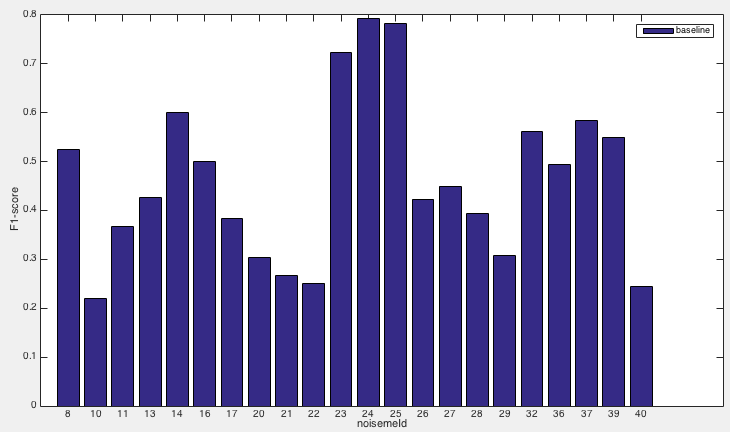
\includegraphics[scale=0.45]{figure/baseline.png}
\caption{The mean F1-score of the baseline.}
\label{fig:baseline}
\end{figure}

Then we conducted several experiments in which we tried to beat the baseline. 
In experiment 1, we used only the automatically generated data to train the classifiers and test on the 40\% manually labeled data. 
The result is in Figure \ref{fig:fOnlyAuto} . As we can see, the F1-scores of these classifiers are far lower than the baseline.

We think there are two reasons for it. 
The first one could be that the training set constructed from the automatically labeled data has low accuracy.Therefore, the classifiers trained on these also has low accuracy.The second reason may be that the baseline classifiers are trained and tested on the same set of data,while the new classifiers are trained and tested on two different sets of data (trained on automatically labeled data and tested on manually labeled data). These two sets of data can be very different.

\begin{figure}[h!]
\centering
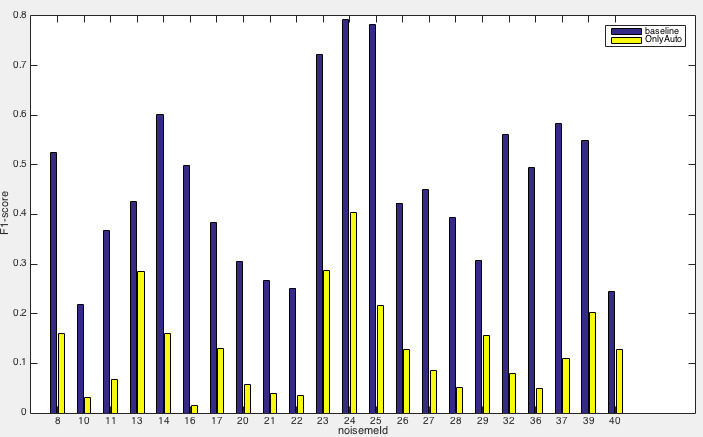
\includegraphics[scale=0.45]{figure/fOnlyAuto.png}
\caption{The mean F1-score of the baseline.}
\label{fig:fOnlyAuto}
\end{figure}

In experiment 2, we combined the manually labeled data and the automatically generated data. 60\% of manually labeled data was randomly selected and combined with automatically generated data(using all of the 5167 correlations) to train the classifiers. %So the training set is 6h * 0.6 + 13.5h. 
The result is in Figure \ref{fig:fmanuAndAuto}.  The result is almost the same as the baseline, which indicate that the training set constructed from automatically generated data does not help to improve the accuracy.The reason may be that the new training set we build has too much noise because we use all the correlations we got. The correlations with low scores may introduce noises into training data.

\begin{figure}[h!]
\centering
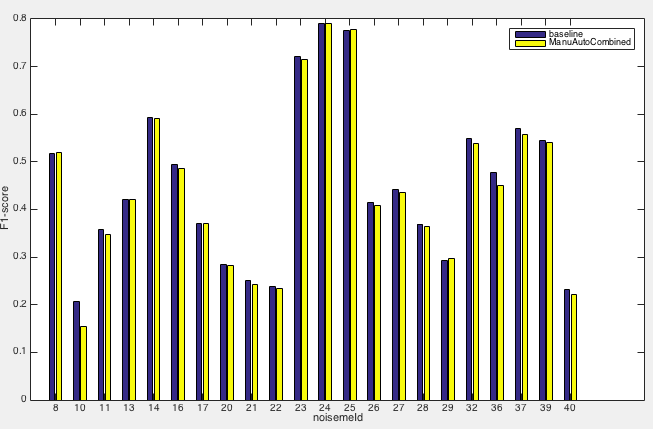
\includegraphics[scale=0.45]{figure/fmanuAndAuto.png}
\caption{The mean F1-score of the baseline and exp2.}
\label{fig:fmanuAndAuto}
\end{figure}

Therefore,in experiment 3, we inspected the effect of different sets of correlations on the performance of the classifiers.In each experiment, top 5000, 3000 and 2000 correlations are selected. 
The result is showed in figure\ref{fig:diffCorrelations}.

There is no much difference between these experiments. We guess the reason may be that even the high ranking correlations have low accuracy(Since we just looked over the TOP 20 correlations and there are some correlations does not make any sense). If the image concepts are not correct, then there is no way that the correlations will be in high quality. So we designed the next experiment to test our conjecture.

\begin{figure}[h!]
\centering
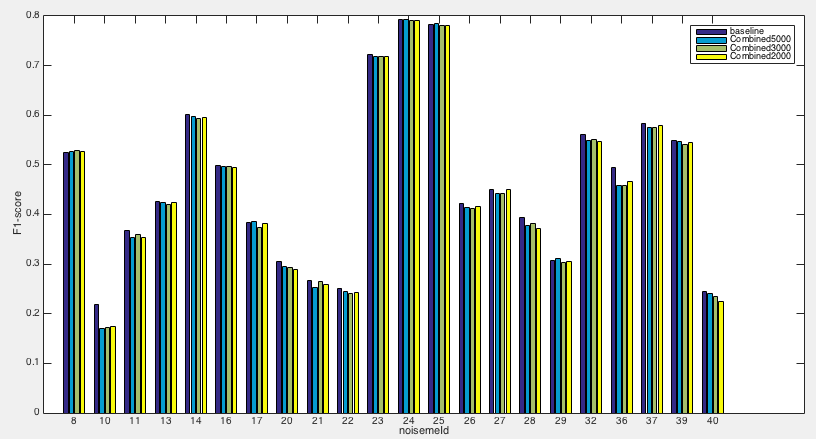
\includegraphics[scale=0.45]{figure/diffCorrelations.png}
\caption{The mean F1-score of the baseline.}
\label{fig:diffCorrelations}
\end{figure}
 
In experiments 4, we tried to improve the quality of the correlations by increasing the accuracy of the image concepts.
Only image concepts with accuracy 80\%+ were selected, which led to 1,256 correlations. And,
since there are less correlations, in order to get the same amount of training data as previous experiments, we changed the way of selecting training set to select contiguous windows of length 5s with the same noiseme label(The second definition of related audio windows as illustrated in Section III-D).
The result is showed in figure \ref{fig:newCombined}. 

We found that 15 out of 22 classifiers were improved.The maximum increase of F1 score is 0.072 (29\%). And average increase of F1 score is 0.024(6.9\%). 

This experiment shows that high quality correlations plays a key role at improving the performance of the detectors.And the high accuracy image concept lead to high quality correlations.

\begin{figure}[h!]
\centering
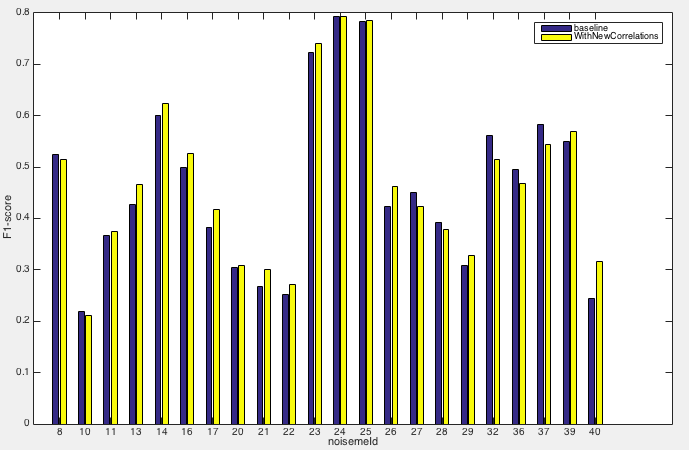
\includegraphics[scale=0.45]{figure/newCombined.png}
\caption{The mean F1-score of the baseline and exp4.}
\label{fig:newCombined}
\end{figure}

After proving the effectiveness of the methods in this experiment, we tried to figure out whether it's because of the less correlations or of using different definition of related audio windows. 
But when we tried to construct training set using the second definition of related audio windows and .


\label{section:results}

% needed in second column of first page if using \IEEEpubid
%\IEEEpubidadjcol

% An example of a floating figure using the graphicx package.
% Note that \label must occur AFTER (or within) \caption.
% For figures, \caption should occur after the \includegraphics.
% Note that IEEEtran v1.7 and later has special internal code that
% is designed to preserve the operation of \label within \caption
% even when the captionsoff option is in effect. However, because
% of issues like this, it may be the safest practice to put all your
% \label just after \caption rather than within \caption{}.
%
% Reminder: the "draftcls" or "draftclsnofoot", not "draft", class
% option should be used if it is desired that the figures are to be
% displayed while in draft mode.
%
%\begin{figure}[!t]
%\centering
%\includegraphics[width=2.5in]{myfigure}
% where an .eps filename suffix will be assumed under latex, 
% and a .pdf suffix will be assumed for pdflatex; or what has been declared
% via \DeclareGraphicsExtensions.
%\caption{Simulation Results}
%\label{fig_sim}
%\end{figure}

% Note that IEEE typically puts floats only at the top, even when this
% results in a large percentage of a column being occupied by floats.


% An example of a double column floating figure using two subfigures.
% (The subfig.sty package must be loaded for this to work.)
% The subfigure \label commands are set within each subfloat command, the
% \label for the overall figure must come after \caption.
% \hfil must be used as a separator to get equal spacing.
% The subfigure.sty package works much the same way, except \subfigure is
% used instead of \subfloat.
%
%\begin{figure*}[!t]
%\centerline{\subfloat[Case I]\includegraphics[width=2.5in]{subfigcase1}%
%\label{fig_first_case}}
%\hfil
%\subfloat[Case II]{\includegraphics[width=2.5in]{subfigcase2}%
%\label{fig_second_case}}}
%\caption{Simulation results}
%\label{fig_sim}
%\end{figure*}
%
% Note that often IEEE papers with subfigures do not employ subfigure
% captions (using the optional argument to \subfloat), but instead will
% reference/describe all of them (a), (b), etc., within the main caption.


% An example of a floating table. Note that, for IEEE style tables, the 
% \caption command should come BEFORE the table. Table text will default to
% \footnotesize as IEEE normally uses this smaller font for tables.
% The \label must come after \caption as always.
%
%\begin{table}[!t]
%% increase table row spacing, adjust to taste
%\renewcommand{\arraystretch}{1.3}
% if using array.sty, it might be a good idea to tweak the value of
% \extrarowheight as needed to properly center the text within the cells
%\caption{An Example of a Table}
%\label{table_example}
%\centering
%% Some packages, such as MDW tools, offer better commands for making tables
%% than the plain LaTeX2e tabular which is used here.
%\begin{tabular}{|c||c|}
%\hline
%One & Two\\
%\hline
%Three & Four\\
%\hline
%\end{tabular}
%\end{table}


% Note that IEEE does not put floats in the very first column - or typically
% anywhere on the first page for that matter. Also, in-text middle ("here")
% positioning is not used. Most IEEE journals use top floats exclusively.
% Note that, LaTeX2e, unlike IEEE journals, places footnotes above bottom
% floats. This can be corrected via the \fnbelowfloat command of the
% stfloats package.

\section{Conclusion}
We can found informative noiseme-image label correlations based on statistical approaches.
With the benefit of these correlations, we can use an image label as an evidence of an automatically generated noiseme label, select those sound snippets as new training data to enrich the training dataset, and get better noiseme detectors.From the experiments, we get the conclusion that the quality of discovered correlations matters.Image concept accuracy is a bottleneck.

\section{Group Contribution}
Tianyu Xu proposed and implemented all the algorithms related to noiseme-image correlations, i.e. correlation discovering, correlation fusion, correlation refinement, and new training set construction. Liping Xiong designed and conducted all the experiments, and gave detailed analysis on them. As for the report, each person is in charge of his/her own part. Overall, Tianyu and Liping have similar workload in this project.

\section*{Acknowledgment}
We want to thank Professor Florian Metze for his detailed and patient guidance during this semester. We also want to thank Shoou-I Yu, who provides the accuracy information of image concepts, and Shicheng Xu, who provides the image concept hierarchy data.

\bibliographystyle{IEEEtran}
\bibliography{ref}

\end{document}